\documentclass[12pt]{article}
\usepackage[margin=0.75in]{geometry}
\usepackage{graphicx}
\setlength{\parindent}{0mm}

\begin{document}

{\centering
\large Physics 1111: Lab 03 \par
\large Projectile Motion \par
}
\hfill \break \vspace{-4mm}

In this lab you will be using the Interactive Physics (IP) software to simulate various kinds of two-dimensional motion and comparing the results to calculations.
Note that you can work from home through your web browser by going to my.ung.edu $\rightarrow$ Remote Access $\rightarrow$ Virtual Lab $\rightarrow$ Download Client $\rightarrow$ HTML 5 Browser $\rightarrow$ VMware Horizon HTML Access and logging in.
As always, do not copy exactly the examples given in these instructions.
Note that it may be possible to use the “guess and check” method in this lab to get approximately correct results; do not do this!
You must show all of your calculations.

Setup:
\begin{enumerate}
\item Open IP
\item Click View $\rightarrow$ Workspace and check ``Grid Lines'' and ``X,Y Axes''
\item Pan the screen so the origin is near the bottom left
\end{enumerate}

\underline{\textbf{Part 1}} \par
\begin{itemize}
\item Use the rectangle tool to create a floor and anchor it.
\item Use the circle tool to create a small circle, drag it to some height above the floor, and give it some velocity in the y-direction (right click the circle to adjust its values); keep $v_x = 0$ for now.
\item Create a second circle at a different height.
Calculate the necessary initial y-velocity so the two circles hit the floor at the same time.
Give the second circle this initial y-velocity.
\item Use the Windows ``Snipping Tool'' to take a screen shot of your initial conditions. (see fig.~\ref{fig:fig1})
\item Select both circles and click Windows $\rightarrow$ Appearance and check ``Track outline''.
Note: additional tracking settings are under World.
Run the simulation until both circles hit the floor.
Take another screenshot to show that your calculations were correct. (see fig.~\ref{fig:fig2})
\item Restart the simulation (clear the tracks by clicking World $\rightarrow$ Erase Track).
Give the circles some random (but reasonable) x-velocity to show they still hit the floor at the same time.
Run the simulation and take another screenshot. (see fig.~\ref{fig:fig3})
\end{itemize}
%
\begin{figure}[!h]
\centering
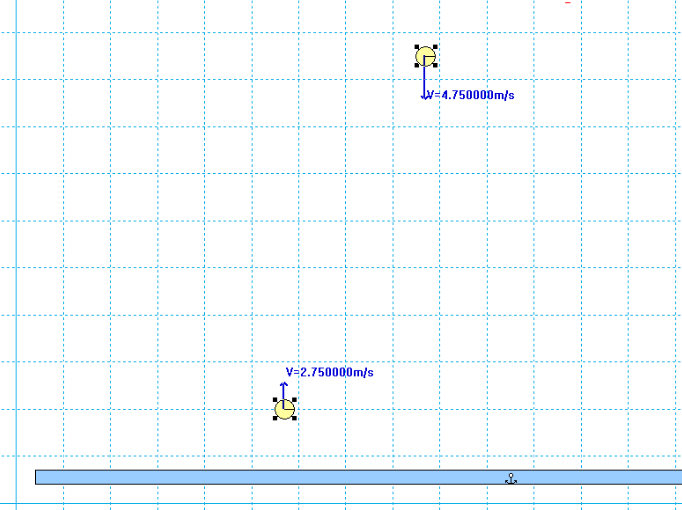
\includegraphics[scale=0.35]{figures/fig1.png}
\caption{Initial conditions.}
\label{fig:fig1}
\end{figure}
%
\begin{figure}[!h]
\centering
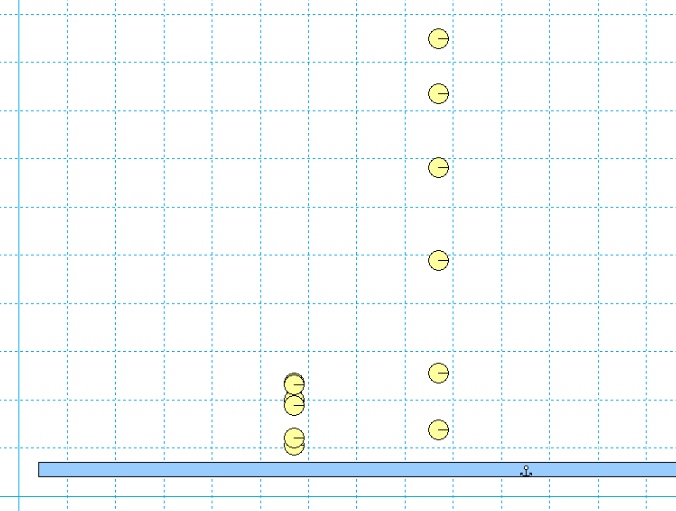
\includegraphics[scale=0.35]{figures/fig2.png}
\caption{1-D motion.}
\label{fig:fig2}
\end{figure}
%
\begin{figure}[!h]
\centering
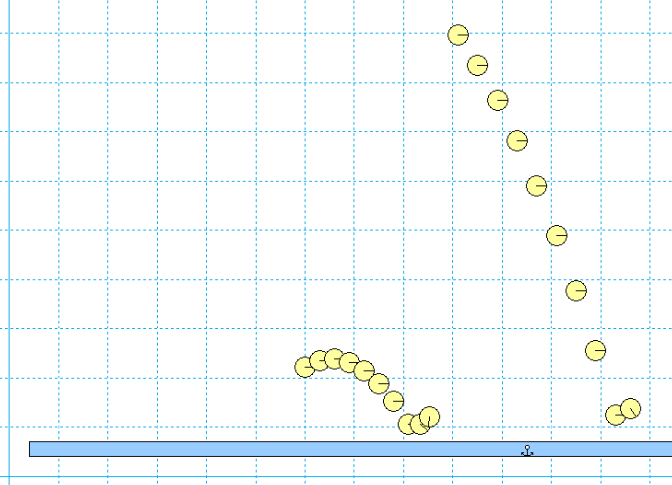
\includegraphics[scale=0.35]{figures/fig3.png}
\caption{Projectile motion.}
\label{fig:fig3}
\end{figure}

\underline{\textbf{Part 2}} \par
\begin{itemize}
\item Using similar techniques as in Part 1, design an experiment where a projectile collides with a freely falling object.
Show relevant screen shots. (see figures~\ref{fig:fig2_1}~and~\ref{fig:fig2_2})
\end{itemize}
%
\begin{figure}[!h]
\centering
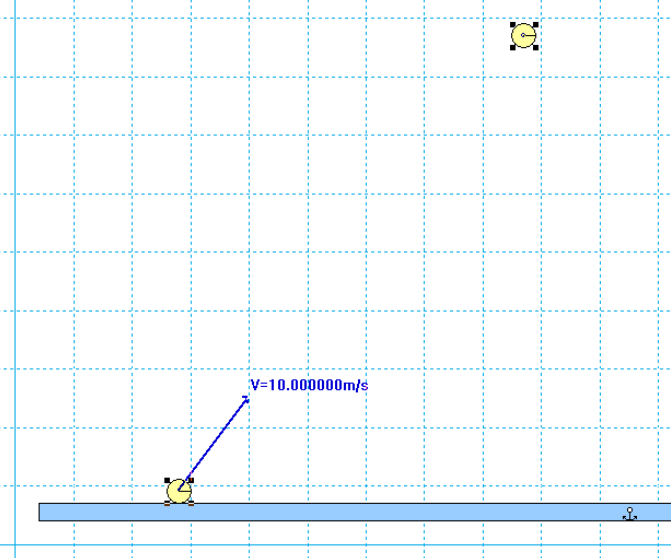
\includegraphics[scale=0.35]{figures/fig2_1.png}
\caption{Part 2 initial conditions.}
\label{fig:fig2_1}
\end{figure}
%
\begin{figure}[!h]
\centering
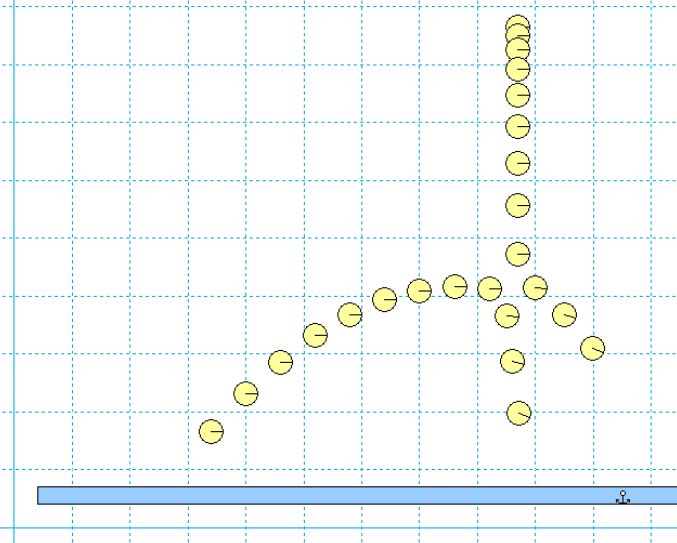
\includegraphics[scale=0.35]{figures/fig2_2.png}
\caption{Part 2 result.}
\label{fig:fig2_2}
\end{figure}


\end{document}
